\documentclass{amsart}
\usepackage[russian]{babel}
\usepackage{latexsym}
\usepackage{amssymb}
\usepackage{amsmath}
\usepackage{underscore}
\usepackage{mathdots}
\usepackage{xcolor}
\usepackage{graphicx}
\usepackage[utf8]{inputenc}
\usepackage{adjustbox}
\usepackage{hyperref}
\usepackage{algorithmic}

\newtheorem{theorem}{Теорема}[section]
\newtheorem{lemma}[theorem]{Lemma}
\newtheorem{proposition}[theorem]{Proposition}
\newtheorem{corollary}[theorem]{Corollary}

\theoremstyle{definition}
\newtheorem{definition}[theorem]{Definition}
\newtheorem{example}[theorem]{Example}
\newtheorem{xca}{Задача}

\theoremstyle{remark}
\newtheorem{remark}[theorem]{Remark}

\numberwithin{equation}{section}

\newcommand{\frc}[2]{\raisebox{2pt}{$#1$}\big/\raisebox{-3pt}{$#2$}}  

\begin{document}
\sloppy

Если наш датасет таков, что все признаки целочисленные и вещественные, нет пропущенных значений и других приятных сюрпризов, то матрица объекты-признаки --- это просто матрица, к которой можно пробовать применять инструменты из линейной алгебры, а среди таковых весьма полезными оказываются матричные разложения, то есть различные способы представить матрицу в виде произведения двух или более матриц, обычно специального вида. Такие разновидности, как LU-разложение, QR-разложение, разложение Холецкого вы несомненно встретите, если откроете код любой библиотеки численной линейной алгебры, но суждено ли матричным разложениям играть роль только лишь винтиков и шестерёнок, запрятанных внутри инструментов машинного обучения, или какие-то из них и сами по себе могут помочь вам анализировать данные? На этот вопрос мы попробуем ответить в данном разделе. Но прежде, чем переходить к конкретным методам, мы разберёмся, к каким моделям данных можно прийти, разложив матрицу в произведение.

\bigskip

\bigskip

\section{Итак, я разложил матрицу в произведения --- и что же?}

Предположим, что нашу матрицу объекты-признаки $X$ мы представили в виде произведения (или, более общо, приблизили в каком-либо смысле таким произведением):
$$\underset{N\times D}{\operatorname{X}} \sim \underset{N\times R}{\operatorname{B}} \cdot \underset{R\times D}{\operatorname{C}}$$
где внизу указаны размеры матриц (то есть в нашем датасете $N$ и $D$ признаков). Что это может означать?

\subsection{Смесь признаков} Мы считаем, что каждый из $D$ признаков нашего исходного датасета --- это смесь (то есть линейная комбинация) $R$ скрытых (латентных) признаков:

\begin{center}
\adjustimage{max size={0.9\linewidth}{0.6\paperheight}}{Decomp1.png} 
\end{center}

По сути это одна из самых простых моделей с латентными переменными, в которой исходные признаки выражаются через латентные линейным образом. Если $R < D$, то мы получаем приближённое описание нашего датасета с помощью меньшего количества признаков. На уровне объектов каждый объект $x_i$ ($D$-мерная строка) приобретает латентное  представление $z_i$ ($R$-мерная строка), с которой он связан соотношением $x_i = z_i\textcolor{green}{C}$.

Точность аппроксимации можно измерять по-разному; наиболее популярной (в силу вычислительной простоты) является норма Фробениуса $||A||_{fro}^2 = \sum_{i,j}A_{ij} = \mathrm{tr}(A^TA)$ --- соответствующую модель называют \textcolor{blue}{анализом главных компонент, или PCA (Principal Component Analysis)}.

\subsection{А если мы хотим получить поменьше признаков?} Мы можем захотеть описать наш датасет меньшим чем $D$ количеством признаков (а может быть, и вообще каким-то весьма маленьким). У нас может быть несколько причин для этого; например:
\begin{itemize}
\item Признаков очень много, и мы боимся, что обучение на них будет занимать очень много времени или что в процессе обучения нам потребуется слишком много оперативной памяти;
\item Мы считаем, что в данных есть шум или что часть признаков связаны соотношением приближённой линейной зависимости --- иными словами, мы уверены, что значительную часть информации можно закодировать меньшим числом признаков;
\end{itemize}
Мы уже обсуждали, что это можно получить, построив приближённое разложение
$$\underset{N\times D}{\operatorname{X}} \sim \underset{N\times T}{\operatorname{B}} \cdot \underset{T\times D}{\operatorname{C}}$$

\textit{Математика помогает}. Матрица имеет ранг $T$ тогда и только тогда, когда она представляется в виде $\underset{N\times S}{\operatorname{B}} \cdot \underset{S\times D}{\operatorname{C}}$ для $S = T$ и не представляется в таком виде для меньших $S$.

Доказывать это мы не будем, но подметим, что \textcolor{blue}{приблизить датасет линейной смесью $T$ признаков --- это то же самое, что приблизить матрицу $X$ матрицей $\hat{X}$ ранга $T$}.

\textit{Качество приближения}. Нам, конечно же, хочется, чтобы приближение было наилучшим --- скажем, в том смысле, чтобы разность $X - BC$ была минимальной в каком-либо смысле. Можно предложить много разных метрик; остановимся на двух:
\begin{itemize}
\item \textcolor{blue}{Норма Фробениуса}. Представим, что матрица $A = (X - BC)$ --- это просто вектор из $N\times D$ чисел, который зачем-то записали в виде прямоугольной таблицы. Тогда его норму можно записать в виде
$$||A||_{fro} = \sqrt{\sum_{i,j}a_{ij}^2} = \mathrm{tr}\left(A^TA\right)$$
Эту норму (а точнее, её квадрат) легко оптимизировать.
\item \textcolor{blue}{Операторная  l2-норма}. Вычислять её тяжко, а уж оптимизировать вообще непонятно так, зато звучит круто. Идея в том, что отображения можно сравнивать в зависимости от того, как оно действует на векторы: чем больше оно умеет удлинять векторы --- тем оно ``больше'':
$$||A||_2 = \sup\left\{\frac{|Av|}{|v|}\mid v\in\mathbb{R}^D\right\}$$
Поскольку $\frac{|A(\lambda v)|}{|\lambda v|} = \frac{|Av|}{|v|}$, достаточно брать супремум только по векторам единичной длины, то есть по единичной сфере. Так как это компакт, непрерывная функция $v\mapsto |Av|$ достигает на нём своего максимального значения, то есть мы можем переписать
$$||A||_2 = \sup\left\{|Av|\mid v\in\mathbb{R}^D,\,|v| = 1\right\}$$
\end{itemize}

\subsection{Смесь объектов} Мы считаем, что каждый из $N$ объектов нашего исходного датасета --- смесь (то есть линейная комбинация) $R$ скрытых объектов:

\begin{center}
\adjustimage{max size={0.8\linewidth}{0.6\paperheight}}{Decomp2.png} 
\end{center}

Такая интерпретация может быть полезна, например, в ситуации, когда объекты --- это записи с каждого из нескольких микрофонов в помещении, признаки --- фреймы, а скрытые объекты --- это голоса отдельных людей.

Также данную модель можно интерпретировать как что-то вроде поиска типичных объектов.

\subsection{Отдельные представления для объектов и признаков} Эту интерпретацию лучше всего пояснить на примере. Пусть объекты нашего датасета соответствуют пользователям интернет-магазина, а признаки --- товарам, причём в клетке с индексом $(i,j)$ записана единица, если пользователь интересовался товаром, и ноль --- если нет (или, в более общей ситуации, рейтинги, которые пользователи ставят товарам).

\begin{center}
\adjustimage{max size={0.8\linewidth}{0.6\paperheight}}{Decomp3.png} 
\end{center}

При перемножении матриц $B$ и $C$ на $(i, j)$-м месте произведении стоит скалярное произведение $i$-й строки $B$ и $j$-го столбца $C$. Таким образом, степень релевантности товара пользователю моделируется скалярным произведением (напрашивается сравнение с косинусным расстоянием) вектора, представляющего $i$-го пользователя, и вектора, представляющего $j$-й товар.

\begin{center}
\adjustimage{max size={0.8\linewidth}{0.6\paperheight}}{Decomp4.png} 
\end{center}

Заметим ещё, что $R$ координат вектора, ответчающего пользователю, равно как и $R$ координат вектора, отвечающего товару, можно рассматривать как $R$ латентных признаков, которые в идеальном мире являются интерпретируемыми и характеризуют <<сродство>> пользователя и товара с некоторым аспектом бытия:

\begin{center}
\adjustimage{max size={0.8\linewidth}{0.6\paperheight}}{Decomp6.png} 
\end{center}

\section{Но матрицы в разложении обычно не абы какие --- так какие из разновидностей могут быть полезны?}

Во всех известных вам матричных разложениях к отдельным сомножителям предъявляются определённые требования: симметричность, треугольность, ортогональность --- некоторые из них (скажем, симметричность) не имеют физического смысла ни в одной из указанных выше интерпретаций. Но одно оказывается полезным.

\subsection{Ковариация и дисперсия признаков} Для начала --- и это важно --- \textcolor{blue}{предположим, что матрица $\textcolor{blue}{X}$ центрирована по столбцам}, то есть среднее в каждом из столбцов (=признаков) равно нулю (если это не так, то вычтем из каждого столбца его среднее).

Теперь матрица ковариации признаков может быть с точностью до константы оценена как $X^TX$:

\begin{center}
\adjustimage{max size={0.8\linewidth}{0.6\paperheight}}{Decomp5.png} 
\end{center}

И мы видим: \textcolor{blue}{$i$-й и $j$-й столбцы матрицы $X$ ортогональны тогда и только тогда, когда соответствующие признаки не коррелированы}.

При этом \textcolor{blue}{$(i,i)$-й диагональный элемент матрицы $X^TX$ --- это дисперсия $i$-го признака}.

\subsection{Вывод: матрица, ортонормированная по столбцам, отвечает датасету, в котором признаки не коррелированы и имеют единичную дисперсию}

\section{Сигнулярное разложение}

С помощью сингулярного разложения можно перейти от $D$ исходных признаков к потенциально небольшому количеству ``самых важных'', по-быстрому визуализовать данные или построить простенькую рекомендательную систему. Конечно, глубинные автоэнкодеры, TSNE или DMMS справятся с этим гораздо лучше, но если данных относительно немного или если хочется что-нибудь быстро попробовать ``на коленке'', старое доброе сингулярное разложение всегда подставит плечо.

\subsection{Математическое определение} \textcolor{blue}{Сингулярным разложением} матрицы $X$ называется разложение
$$X = \textcolor{orange}{U}\textcolor{green}{\Sigma}\textcolor{magenta}{V^T},$$
где $\textcolor{orange}{U}$ и $\textcolor{magenta}{V}$ --- матрицы, ортонормированные по столбцам, а $\textcolor{green}{\Sigma} = \mathrm{diag}(\textcolor{green}{\sigma_1},\textcolor{green}{\sigma_2},\ldots)$ --- диагональная матрица, у которой $\textcolor{green}{\sigma_1}\geqslant\textcolor{green}{\sigma_2}\geqslant\ldots\geqslant\textcolor{green}{\sigma_R}>\textcolor{green}{\sigma_{R+1}}=0$. Числа $\textcolor{green}{\sigma}_i$ называются \textcolor{green} {сингулярными числами}, а столбцы$\textcolor{orange}{U}$ и $\textcolor{magenta}{V}$ --- \textcolor{orange}{левыми} и \textcolor{magenta}{правыми} сингулярными векторами соответственно (их алгебраический смысл станет ясен чуть ниже).

Сингулярное разложение можно записать в полном или в усечённом виде:

\begin{center}
\adjustimage{max size={0.8\linewidth}{0.6\paperheight}}{SVD1.png} 
\end{center}

Пара предостережений по поводу ортогональности по столбцам:

\begin{center}
\adjustimage{max size={0.8\linewidth}{0.6\paperheight}}{SVD2.png} 
\end{center}

Ясно, что хранить полное разложение нет смысла: ведь в нём нет ничего нужного для восстановления исходной матрицы, а бесполезные блоки будут лишь занимать память.

По-английски сингулярное разложение называется SVD (singular value decomposition), и мы будем активно использовать эту аббревиатуру.

\textit{Если вы не любите математику, можете пропустить}. С точки зрения математики сингулярное разложение говорит следующее. Пусть $X$ --- матрица линейного отображения $\varphi:\mathbb{R}^D\longrightarrow\mathbb{R}^N$. Тогда найдётся ортонормированый базис $\textcolor{magenta}{v_1},\dots,\textcolor{magenta}{v_D}$ в пространстве $\mathbb{R}^D$ и ортонормированый базис $\textcolor{orange}{u_1},\dots,\textcolor{orange}{u_N}$ в пространстве $\mathbb{R}^N$, в которых действие оператора записывается следующим образом:
\begin{align*}
\varphi(\textcolor{magenta}{v_1}) &= \textcolor{green}{\sigma_1}\textcolor{orange}{u_1},\\
\vdots\\
\varphi\textcolor{magenta}{(v_R}) &= \textcolor{green}{\sigma_r}\textcolor{orange}{u_R},\\
\varphi(\textcolor{magenta}{v_{R+1}}) &= 0,\\
\vdots\\
\varphi(\textcolor{magenta}{v_D}) &= 0
\end{align*}
(знатоки функционального анализа могут узнать в этом частный случай теоремы Гильберта-Шмидта).

\textit{Сингулярное разложение и операторная l2-норма}. Можно показать, что $||A||_2$, эта самая операторная l2-норма матрицы, равна $\sigma_1^2$ --- квадрату наибольшего сингулярного числа.

\textit{Сингулярное разложение и норма Фробениуса}. Можно показать, что 
$$||A||_{fro} = \sqrt{\sum_i\sigma_i^2}$$

\textit{Контрольный вопрос}. Единственно ли сингулярное разложение матрицы? Давайте сразу считать, что речь об усечённом разложении.

\textit{Ответ} (пожалуйста, подумайте сперва сами, а потом читайте). Есть очень простой источник неоднозначности: если $\varphi(\textcolor{magenta}{v_i}) = \textcolor{green}{\sigma_1}\textcolor{orange}{u_i}$, то и $\varphi(\textcolor{magenta}{-v_i}) = \textcolor{green}{\sigma_1}\textcolor{orange}{-u_i}$; при этом умножение вектора на $(-1)$ не попортит ортонормированности базиса. Иными словами, мы можем одновременно поменять знаки $i$-х столбцов матриц $\textcolor{orange}{U}$ и $\textcolor{magenta}{V}$ (без транспонирования!) без ущерба для разложения.

Есть и более тонкие, хотя и весьма частные, ситуации. Можете ли вы, например, указать несколько различных сингулярных разложений матрицы $E$? Да-да, для неё сингулярное разложение максимально неоднозначно. Можете ли вы теперь придумать не скалярную матрицу, у которой были бы различные SVD, отличающиеся не только знаками столбцов матриц $\textcolor{orange}{U}$ и $\textcolor{magenta}{V}$?

\subsection{Теоретико-вероятностная интерпретация SVD} Если $X =\textcolor{orange}{U}\textcolor{green}{\Sigma} \textcolor{magenta}{V^T}$ (рассмотрим сейчас не усечённое, а полное разложение, в котором матрицы $\textcolor{orange}{U}$ и $\textcolor{magenta}{V}$ квадратные ортогональные), то 
$$X^TX = \textcolor{magenta}{V}\underbrace{\textcolor{green}{\Sigma^T}}\underbrace{\textcolor{orange}{U^T}\cdot \textcolor{orange}{U}}_{=E}\textcolor{green}{\Sigma} \textcolor{magenta}{V^T} =
\textcolor{magenta}{V}\textcolor{green}{\Sigma}^T\textcolor{green}{\Sigma} \textcolor{magenta}{V^T}$$
Отметим, что в рассматриваемой ситуации $\textcolor{green}{\Sigma}$ не обязательно квадратная, и поэтому нельзя написать, что $\textcolor{green}{\Sigma}^T\textcolor{green}{\Sigma}=\textcolor{green}{\Sigma}^2$; тем не менее, $\textcolor{green}{\Sigma}^T\textcolor{green}{\Sigma}$ --- это квадратная матрица с числами $\textcolor{green}{\sigma_1}^2,\textcolor{green}{\sigma_2}^2,\ldots$ на диагонали.

\medskip

\textit{Контрольный вопрос}/ Точно так же мы можем вычислить $XX^T = \textcolor{orange}{U}^T\textcolor{green}{\Sigma}\textcolor{green}{\Sigma}^T\textcolor{orange}{U}$, где опять-таки $\textcolor{green}{\Sigma}\textcolor{green}{\Sigma}^T$ --- квадратная матрица с числами $\textcolor{green}{\sigma_1}^2,\textcolor{green}{\sigma_2}^2,\ldots$ на диагонали. И всё бы хорошо, но если $\textcolor{green}{\Sigma}$ не квадратная, матрицы $\textcolor{green}{\Sigma}^T\textcolor{green}{\Sigma}$ и $\textcolor{green}{\Sigma}\textcolor{green}{\Sigma}^T$ имеют разные размеры. Так в чём же подвох?

\medskip

Как бы то ни было, в (ортогональном!) базисе из (ортогональных!) столбцов $\textcolor{magenta}{V}$ матрица $X^TX$ приводится к диагональному виду с числами $\textcolor{green}{\sigma_1}^2,\textcolor{green}{\sigma_2}^2,\ldots$ на диагонали.

Теперь представим, что наши объекты $x_1,x_2,\ldots,x_N$ выбраны из $D$-мерного нормального распределения
$$p(x_i) = \frac{1}{(2\pi)^{D/2}|C|^{1/2}}e^{-\frac12(x_i - \mu)C^{-1}(x_i - \mu)^T}$$
где $\mu$ --- вектор средних, а $C$ --- матрица ковариации. Это, в частности, значит, что облако точек представляет из собой нечто вроде эллипсоида в $D$-мерно пространстве с центром $\mu$.

Предположим, что $\mu = 0$ (все признаки центрированы); тогда оценкой матрицы ковариации признаков является матрица $\frac1n X^TX$. Допустим, что эта оценка точная, тогда разложение $X^TX = \textcolor{magenta}{V}\textcolor{green}{\Sigma}^T\textcolor{green}{\Sigma} \textcolor{magenta}{V}^T$ даёт нам аналогичное разложение $C = \textcolor{magenta}{V}(\frac1n\textcolor{green}{\Sigma}^T\textcolor{green}{\Sigma}) \textcolor{magenta}{V}^T$. Теперь замена координат $x = z\textcolor{magenta}{V}^T$ (с матрицей замены $\textcolor{magenta}{V}$ --- то есть переход происходит в базис из столбцов матрицы $\textcolor{magenta}{V}$) даёт нам
$$p(x_i) = \mathrm{const}\cdot \exp\left(-\frac12\cdot\textcolor{red}{x_i}\cdot \textcolor{blue}{C^{-1}}\cdot \textcolor{cyan}{x_i^T}\right)$$
Обратите внимание, что $x_i$ и $x_i^T$ стоят в формуле на непривычных местах, как будто их перепутали, но нет --- просто $x_i$ у нас является строкой, а не столбцом.
$$p(z) = \mathrm{const}\cdot \exp\left(-\frac12\cdot\textcolor{red}{z_i}\underbrace{\textcolor{red}{V^T}\cdot \textcolor{blue}{V}}_{=E}\textcolor{blue}{(n\Sigma^{-1}\Sigma^{-T})}\underbrace{\textcolor{blue}{V^T}\cdot \textcolor{cyan}{V}}_{=E}\textcolor{cyan}{z_i^T})\right)=$$
$$= \mathrm{const}\cdot \exp\left(-\frac{n}2z_i\Sigma^{-1}\Sigma^{-T}z_i^T)\right)=\mathrm{const}\cdot \exp\left(-\frac{n}2\left(\frac1{\sigma_1^2}z_{i1}^2 + \frac1{\sigma_2^2}z_{i2}^2 + \ldots\right)\right)=$$
$$=p(x'_{i1})\cdot\ldots\cdot p(x'_{iD})$$
Итак, если наши данные взяты из многомерного нормального распределения, после перехода к базису из столбцов $\textcolor{magenta}{V}$ новые координаты становятся независимыми; вместе с тем это соответствует переходу к главным осям ковариационной матрицы --- и геометрически стобцы $V$ соответствуют главным осям эллипсоида-облака точек.

\begin{center}
\adjustimage{max size={0.5\linewidth}{0.6\paperheight}}{SVD3.png} 
\end{center}

\subsection{Доказательство существования сингулярного разложения (не читайте, если не хотите)} 

\section{И как же использовать SVD? Вариант 1 --- латентные признаки}

Запишем
$$\underset{N\times D}{\operatorname{X}} = \underset{N\times R}{\operatorname{U\Sigma}} \cdot \underset{R\times D}{\operatorname{V^T}}$$
и вспомним самую первую интерпретацию матричного разложения.

\begin{center}
\adjustimage{max size={0.5\linewidth}{0.6\paperheight}}{SVD4.png} 
\end{center}

Столбцы $U\Sigma$ ортогональны (так как они пропорциональны столбцам ортогональной по столбцам матрицы $U$) --- то есть \textcolor{blue}{латентные признаки не коррелированы}. При этом, поскольку длина каждого из столбцов $U$ равна 1, длины столбцов $U\Sigma$ порпорциональны $\sigma_i$ --- а, значит, \textcolor{blue}{латентные признаки упорядочены по неубыванию дисперсии} (ведь с точностью до константы оценка дисперсии признака --- это квадрат длины вектора его значений).

Заметим, что перед применением SVD признаки лучше центрировать, иначе первая компонента будет указывать в сторону центра масс облака точек (зачем нам это?), а остальные вынуждены будут ей быть ортогональны:

\begin{center}
\adjustimage{max size={0.5\linewidth}{0.6\paperheight}}{SVD5.png} 
\end{center}

\subsection{А если мы хотим получить поменьше признаков?} Мы уже обсуждали, что это можно получить, построив приближение ранга $T$ или, что то же самое, приближённое разложение
$$\underset{N\times D}{\operatorname{X}} \sim \underset{N\times T}{\operatorname{B}} \cdot \underset{T\times D}{\operatorname{C}}$$
для некоторого и желательно небольшого $T$. И тут SVD приходится более чем кстати. 

\textbf{\textcolor{blue}{Теорема Эккарта-Янга}} Наилучшее по норме Фробениуса приближение ранга $T$ --- это 

\begin{center}
\adjustimage{max size={0.8\linewidth}{0.6\paperheight}}{SVD6.png} 
\end{center}

Таким образом, если вы хотите получить $T$ ``самых важных'' признаков, то вы можете использовать SVD. Но что это за признаки? Что именно означают эти слова ``самые важные''? Давайте обратимся к геометрии, которая, как мы помним, тесно связана с теорией вероятностей:

\begin{center}
\adjustimage{max size={0.6\linewidth}{0.6\paperheight}}{SVD7.png} 
\end{center}

\begin{center}
\adjustimage{max size={0.6\linewidth}{0.6\paperheight}}{SVD8.png} 
\end{center}

Если применить SVD к датасету, изображённому на последней картинке, и взять два первых латентных признака, то эллипсоид превратится в эллипс; меньшая из полуосей, похожая на шум, будет забыта, останется две б\'{о}льших. Видим: самое важное для SVD --- это самое масштабное.

\medskip

\textit{А правда ли у нас получится хорошее приближение с помощью $T$ новых признаков?} Посчитаем норму разности. Везде ниже $\textcolor{orange}{U}$ и $\textcolor{magenta}{V}$ --- квадратные ортогональные матрицы; в частности $\textcolor{green}{\Sigma}$ не обязательно квадратная матрица размера $N\times D$.

\begin{center}
\adjustimage{max size={0.6\linewidth}{0.6\paperheight}}{SVD9.png} 
\end{center}

$$||\Delta||_{fro}^2 = \mathrm{tr}\left((\textcolor{orange}{U}\textcolor{green}{\widetilde{\Sigma}}\textcolor{magenta}{V}^T)^T\textcolor{orange}{U}\textcolor{green}{\widetilde{\Sigma}}\textcolor{magenta}{V}^T\right) = 
\mathrm{tr}\left(\textcolor{magenta}{V}\textcolor{green}{\widetilde{\Sigma}}^T\underbrace{\textcolor{orange}{U}^T\textcolor{orange}{U}}_{=E}\textcolor{green}{\widetilde{\Sigma}}\textcolor{magenta}{V}^T\right) =$$
$$=\mathrm{tr}\left(\textcolor{magenta}{V}\textcolor{green}{\widetilde{\Sigma}}^T\textcolor{green}{\widetilde{\Sigma}}\textcolor{magenta}{V}^T\right) = \mathrm{tr}\left(\textcolor{green}{\widetilde{\Sigma}}^T\textcolor{green}{\widetilde{\Sigma}}\underbrace{\textcolor{magenta}{V}^T\textcolor{magenta}{V}}_{=E}\right) = ||\textcolor{green}{\widetilde{\Sigma}}||^2_{fro} = \textcolor{green}{\sigma_{T+1}}^2 + \ldots + \textcolor{green}{\sigma_{R}}^2$$
Аналогичным образом
$$||\Delta||_2 = \textcolor{green}{\sigma_{T+1}}$$
потому что умножение на ортогональную матрицу не меняет операторную $l_2$-норму. Таким образом, если сингулярные значения убывают достаточно медленно (например, линейно), то мы вряд ли сможем приблизить исходную матрицу матрицей маленького ранга с очень хорошей точностью.

\medskip

\textit{Как избавиться от иллюзий}. Сгенерируйте матрицу $100\times100$ с помощью \texttt{np.random.rand} или \texttt{np.random.randn}. Для какого $T$ вы сможете найти матрицу ранга $T$, приближающую исходную с относительной точностью $10^{-6}$?

\medskip

К счастью, в реальных датасетах сингулярные значения убывают достаточно быстро или же нам хватает довольно грубого приближения.

\subsection{Как перейти из исходного признакового пространства в новое (в том числе с меньшим числом признаков) и обратно?}

Допустим, мы построили приближённое разложение ранга $T$:
$$X\sim\textcolor{orange}{\widehat{U}}\textcolor{green}{\widehat{\Sigma}}\textcolor{magenta}{\widehat{V}}^T = 
\textcolor{orange}{U}\cdot\underbrace{\textcolor{green}{\begin{pmatrix}
\sigma_1 &\\
 & \ddots & \\
 & & \sigma_T &\\
& & & 0 & \\
& & & & \ddots\end{pmatrix}}}_{=:\textcolor{green}{\Sigma'}}\cdot\textcolor{magenta}{V}^T$$
Матрица $\textcolor{orange}{\widehat{U}}\textcolor{green}{\widehat{\Sigma}}$ --- это первые $T$ столбцов матрицы $\textcolor{orange}{U}\textcolor{green}{\Sigma'}$, и они же первые $T$ столбцов матрицы $\textcolor{orange}{U}\textcolor{green}{\Sigma} = X\cdot\textcolor{magenta}{V}$. Таким образом, \textcolor{blue}{для перевода объекта $x_i$ в новое признаковое пространство нужно произвести $x_i\mapsto x_i\cdot\textcolor{magenta}{V}$ и взять первые $T$ столбцов или, что то же самое, $x_i\mapsto x_i\cdot\textcolor{magenta}{V[:,:T]}$}.

Теперь пусть задана вектор-строка $z_i$ длины $T$ --- латентное представление, соответствующего некоторому объекту, то есть одна из строк матрицы $\textcolor{orange}{\widehat{U}}\textcolor{green}{\widehat{\Sigma}}$. Тогда точно восстановить исходный $x_i$ мы не сможем: ведь равенство $X\sim\textcolor{orange}{\widehat{U}}\textcolor{green}{\widehat{\Sigma}}\textcolor{magenta}{\widehat{V}}^T$ не точное, но \textcolor{blue}{для приближённого восстановления $x_i$ мы должны произвести $z_i\mapsto z_i\cdot \textcolor{magenta}{\widehat{V}}^T = z_i\cdot\textcolor{magenta}{V[:,:T]}^T$}.


\subsection{На что не способно сингулярное разложение} Сингулярное разложение умеет находить дающие самый существенный вклад в дисперсию линейные комбинации признаков, притом некоррелированные; в случае нормально распределённых данных эти направления оказываются главными осями эллипсоида, которым является облако данных. К сожалению, эта суперспособность SVD столь же охотно превращается в слабость, ведь:
\begin{itemize}
\item Данные не всегда распределены нормальны, они могут обладать сложной геометрией, но SVD будет упрямо искать эллипсоид.
\item Самое важное не всегда самое масштабное. Забыть привести признаки к одному масштабу --- хороший способ выстрелить себе в ногу при работе с сингулярным разложением.
\item Новые признаки не обязаны быть хорошо интерпретируемыми. Линейная комбинация возраста, стажа работы и зарплаты --- это не то, что хотелось бы показывать банковскому регулятору.
\item Выбросы почти наверняка усложнят вам жизнь, хотя, возможно, SVD поможет вам их увидеть.
\end{itemize}

\subsection{Посмотрим кейс: MNIST и путешествие по латентному пространству}

Возьмём большой датасет MNIST, состоящий из чёрно-белых изображений рукописных цифр размера $28\times28$ пикселей (его можно загрузить, к примеру, из \texttt{tensorflow.keras.datasets}), вытянем каждое из изображений в вектор, получив тем самым матрицу размера $60000\times(28\cdot28)$, и применим к этой матрице SVD. Теперь возьмём первые два латентных признака (то есть первые два столбца матрицы $U\Sigma$) --- получается, что каждая рукописная цифра у нас теперь кодируется вектором из двух чисел. Нарисуем на плоскости точки, соответствующие этим векторам (скажем, по 100 из каждого класса, чтобы хоть что-нибудь было понятно):

\begin{center}
%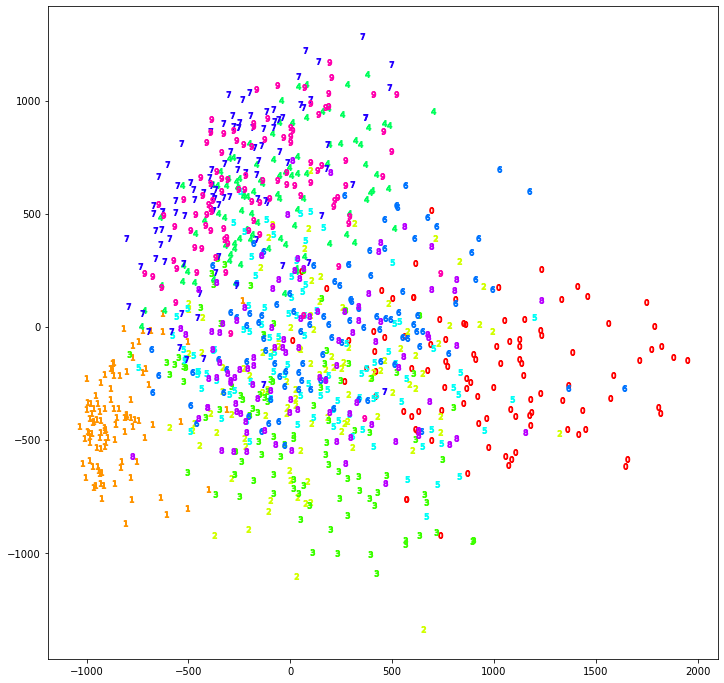
\includegraphics{MNIST-SVD-latent-space.png} 
\adjustimage{max size={0.6\linewidth}{0.6\paperheight}}{MNIST-SVD-latent-space-bad.png}
\end{center}

Что же мы видим? Единицы и нули оказались особенными, то есть уже первые два латентных признака хорошо их различают, правда, с середине какая-то каша. А почему? Да потому, что мы забыли центрировать данные. Давайте перед применением SVD вычтем из каждого признака (то есть из каждого пикселя) его среднее по всем картинками, а потом нарисуем всё заново:

\begin{center}
%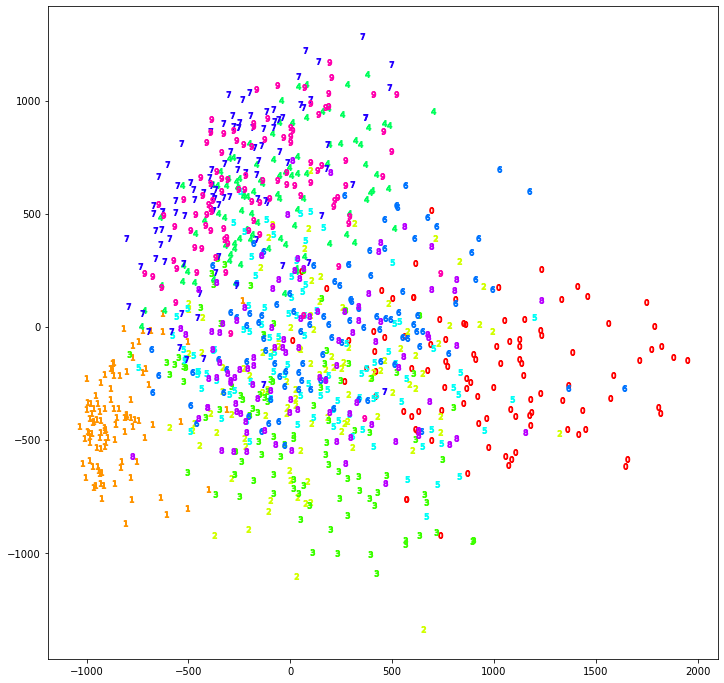
\includegraphics{MNIST-SVD-latent-space.png} 
\adjustimage{max size={0.6\linewidth}{0.6\paperheight}}{MNIST-SVD-latent-space.png} 
\end{center}

Теперь стало получше: например, семёрки, девятки и четвёрки сгуппировались вместе с другой стороны от девяток и троек (собственно говоря, это отражает тот факт, что рукописные написания семёрок, девяток и четвёрок могут быть похожи друг на друга, так и человек не сразу отличит --- а вот с тройкой их спутать намного труднее).

Заметим ещё вот что. В $(28\cdot28)$-мерном пространстве наборов пикселей совсем не каждая точка соответствует какой-то рукописной цифре --- то, что может приходить из реального мира, лежит на некоторой хитрой поверхности в этом пространстве (если выражаться корректнее, то на подмногообразии). Если же мы попробуем нарисовать ``изображения'', лежащие на отрезке, соединяющем два изображения цифр, то получим нечто не слишком интересное:

HERE BE GIF


Одно изображение просто наложилось и затем сменило другое --- скучно! Но если мы сделаем то же самое в двумерном пространстве, образованном первыми двумя латентными признаками SVD, то мы будем получать, может быть, не совсем реалистичные изображения цифр, но что-то явно из мира рукописных символов:

HERE BE GIF

\textit{Контрольный вопрос}. Если $x_1$ --- вектор-строка длины $28\cdot28$, отвечающая первой картинке, $x_2$ --- второй, а $U$, $\Sigma$, $V^T$ --- матрицы из сингулярного разложения, то как получить картинку, соответствующую середине отрезка, соединяющего в пространстве двух первых латентным признаков SVD точки $x_1'$ и $x_2'$, отвечающие этим картинкам?

\subsection{Посмотрим кейс: химический состав рек} Посмотрим на небольшой кусок вот \href{https://data.europa.eu/euodp/en/data/dataset/data_waterbase-rivers-10}{этого датасета}, который доступен для скачивания нигде (ха-ха) и попробуем что-нибудь понять про химических состав рек европейского союза, а заодно соберём шишки, которые могут попасться при визуализации с помощью SVD.

Конечно, сразу хочется нарисовать все объекты датасета в виде точек на плоскости. Мы знаем, что в этом может помочь SVD --- попробуем же! Центрируем признаки --- и рисуем:

\begin{center}
\adjustimage{max size={0.6\linewidth}{0.6\paperheight}}{Rivers-bad-SVD.png} 
\end{center}

Ой, что-то пошло не так. Но почему же?! Наверное, надо хотя бы посмотреть на данные...
\begin{itemize}
\item Объекты имеют вид ``GBPKER0059'', ``GB20227'', ``LVV0120100'' и так далее --- это коды станций, измеряющих состав воды;
\item Признаки имеют вид ``1985 BOD5'', ``1985 Chlorophyll a'', ``1985 Orthophosphates'' и так далее --- тут указан год измерения и показатель;
\item Посмотрев статистики, убеждаемся, что все показатели неотрицательны (то есть уж точно распределены не нормально --- но может, и так сработает); при этом почти все элементы нашей матрицы находятся в пределах 1000, но три значения космически огромны, причём в одном столбце (``2008 Total oxidised nitrogen''; это какие-то греческие станции, с которыми вообще всё странно), и ещё одно тоже очень большое (``2005 Total organic carbon (TOC)'') --- вот они-то и дали нам четыре точки на графике, отличных от начала координат. Кстати говоря, если космически большие значения, по-видимому, являются результатам поломки, то по поводу четвёртого, не столь злостного, выброса есть подозрение, что это реальные значения. Посмотрев в данные, мы видим, что показатель был измерен на станции Zidlochovice, на реке Srvatka ниже Брно --- а, как говорит нам википедия, \textit{As a result of water pollution by communal sewage, the reservoir suffered from an extensive amount of cyanobacteria for a long time}. Так или иначе, все четыре станции мы уберём, чтобы они не портили нам SVD.
\item Один из признаков (``2002 Kjeldahl Nitrogen'') принимает только нулевые значения. Уберём его, чтобы не мешался. 
\end{itemize}

Почистив выбросы в исходных данных, опять центрируем и рисуем:

\begin{center}
\adjustimage{max size={0.6\linewidth}{0.6\paperheight}}{Rivers-SVD-1.png} 
\end{center}

Уже лучше. Попробуем понять, что за вещества внесли вклад в первые два латентных признака. Как это сделать? Латентные признаки --- это столбцы матрицы $U\Sigma = XV$; линейная алгебра говорит нам, что $i$-й столбец произведения $XV$ --- это линейная комбинация столбцов $X$ с коэффициентами из $i$-го столбца $V$. Находим номера самых больших по модулю координат $V$ --- и оказывается, что первые два латентных признака складываются почти сплошь из насыщения воды кислородом, только за разные годы (первый за более старые, второй за чуть более свежие):

\begin{center}
\textbf{First latent feature}

\begin{tabular}{|l|l|}
\hline
Признак & элемент $V$\\
\hline
2001 Oxygen saturation & 0.27\\
\hline
2002 Oxygen saturation & 0.27\\
\hline
2000 Oxygen saturation & 0.26\\
\hline
2004 Oxygen saturation & 0.26\\
\hline
$\vdots$ & $\vdots$\\
\hline
\end{tabular}

\medskip

\textbf{Second latent feature}

\begin{tabular}{|l|l|}
\hline
Признак & элемент $V$\\
\hline
2008 Oxygen saturation & -0.62\\
2007 Oxygen saturation & -0.49\\
2009 Oxygen saturation & -0.45\\
2006 Oxygen saturation & -0.26\\
\hline
$\vdots$ & $\vdots$\\
\hline
\end{tabular}

\end{center}

Неужели насыщение кислородом действительно так важно? Нет, просто мы не отмасштабировали признаки. Оказывается, что насыщение кислородом имеет на порядок больший масштаб, чем многое другое, и потому забивает все остальные признаки. Тем не менее, мы можем попробовать сделать вывод и из имеющейся картинки. По оси у что-то не очень интересное, а по оси х видим большой кластер (напомним, это меньшие значения насыщения воды кислородом в начале 2000-х), содержащий, если проверить, примерно три четверти всех точек, и ещё некоторой размазанный шлейф. Итак, на многих станциях насыщение воды кислородом в начале 2000-х было примерно в одинаковой степени мало --- проверив глазами, обнаруживаем, что там просто нули. Посколько вряд ли это так на самом деле, видимо, стоит сделать вывод, что в первой половине 2000-х насыщение кислородом измерялось из рук вон плохо.

Теперь вдобавок к центрированию поделим каждый признак на его стандартное отклонение и снова нарисуем:

\begin{center}
\adjustimage{max size={0.6\linewidth}{0.6\paperheight}}{Rivers-SVD-2.png} 
\end{center}

Опять видим тесный кластер. При этом первый латентный признак складывается в основном из ``Nitrate'' , ``pH''  и ``Dissolved oxygen'' за разные годы, все с положительными коэффициентами, а второй --- из ``Total ammonium'', ``Total phosphorus'' и ``Kjeldahl Nitrogen'' за разные годы, причём с отрицательными коэффициентами. В частности, справа у нас точки с высоким содержанием нитратов и высокой кислотностью. Среди этих точек:
\begin{itemize}
\item \href{https://en.wikipedia.org/wiki/River_Tame,_West_Midlands}{Река Тейм}, про которую Википедия пишет: ``The Tame was once one of Britain's dirtiest rivers.';
\item Река Кёрёш, про которую тоже можно найти вот такую информацию: ``For some time the municipal government of Kanjiža (to which the mouth of the river belongs) protests about the extreme pollution of the Kereš's water, as it represents the single largest polluter of the Tisa river'';
\item Темза (станция немного выше Лондона).
\end{itemize}
Что ещё можно было бы сделать? Например, мы можем посмотреть распределения признаков и увидеть, что многие из них далеки от нормальных и в целом выиграли бы от логарифмирования --- тогда, возможно, итоговая картинка стала бы красноречивей.

\subsection{Вероятностный PCA} Давайте более подробно обсудим, какую модель данных предполагает PCA. Мы говорим о том, что у каждого $D$-мерного объекта $x_i$ (строки $X$) есть латентное $T$-мерное представление $z_i$ (строка матрицы $\textcolor{orange}{\widehat{U}}$), которое связано с исходным соотношением $x_i \sim z_i\textcolor{green}{\widehat{\Sigma}}\textcolor{magenta}{\widehat{V}}^T$ (да, $\textcolor{green}{\widehat{\Sigma}}$ стоит в необычном месте, но мы скоро увидим, почему). Давайте, как обычно, скажем, что разница --- это изотропный гауссовский шум:
$$x_i\sim z_i\textcolor{green}{\widehat{\Sigma}}\textcolor{magenta}{\widehat{V}}^T + \xi_i,\quad\mbox{где $\xi_i\sim\mathcal{N}(0,\sigma^2E)$}$$
Иными словами,
$$x_i\sim\mathcal{N}(z_i\textcolor{magenta}{\textcolor{green}{\widehat{\Sigma}}\widehat{V}}^T,\sigma^2E)$$
Зададим также априорное распределение $z_i$ как стандартное нормальное: $z_i\sim\mathcal{N}(0,E)$. Тогда $z_i\textcolor{magenta}{V}^T\sim\mathcal{N}(0, \textcolor{magenta}{\widehat{V}}^T\textcolor{green}{\widehat{\Sigma}}^2\textcolor{magenta}{\widehat{V}})$ (вспомните, как преобразуется ковариационная матрица при линейных преобразованиях и не забудьте, что $z_i$ --- строка, а не столбец) и, соответственно $x_i\sim\mathcal{N}(0, \textcolor{magenta}{\widehat{V}}^T\textcolor{green}{\widehat{\Sigma}}^2\textcolor{magenta}{\widehat{V}} + \sigma^2E)$.

Казалось бы, логично. Но правда ли, что модель действительно соответствует PCA? Давайте представим, что вместо $\textcolor{green}{\widehat{\Sigma}}\textcolor{magenta}{\widehat{V}}^T$ у нас стоит некоторая матрица $W^T$ --- будет ли значение $W^T$, подобранное по данным методом максимального правдоподобия, равно $\textcolor{green}{\widehat{\Sigma}}\textcolor{magenta}{\widehat{V}}^T$? И почему, кстати, не просто $\textcolor{magenta}{\widehat{V}}^T$? Если попробовать найти $W$ методом максимального правдоподобия, то мы должны максимизировать
$$\log{p(x_i|W,\sigma)} = -\frac{N}2\log{\det(W^TW + \sigma^2E)} -\frac12\sum_ix_i(W^TW + \sigma^2E)^{-1}x_i^T + \mathrm{const}$$
(вам может показаться, что транспонирование стоит не там --- но снова вспомним, что $x_i$ -- это строка, а не столбец). Заметим, что число равно следу матрицы, состоящей из этого числа, и преобразуем второе слагаемое следующим образом:
$$-\frac12\sum_ix_i(W^TW + \sigma^2E)^{-1}x_i^T = -\frac12\mathrm{tr}\left(\sum_ix_i(W^TW + \sigma^2E)^{-1}x_i^T\right) = $$
$$=-\frac12\mathrm{tr}\left((W^TW + \sigma^2E)^{-1}\cdot\left(\sum_ix_i^Tx_i\right)\right) = -\frac12\mathrm{tr}\left((W^TW + \sigma^2E)^{-1}\cdot X^TX\right)$$
Итак,
$$\log{p(x_i|W,\sigma)} = -\frac{N}2\log{\det(W^TW + \sigma^2E)}  -\frac12\mathrm{tr}\left((W^TW + \sigma^2E)^{-1}\cdot X^TX\right)$$
Найти отсюда $W$ не очень трудно: нужно просто продифференцировать и приравнять к нулю --- но некоторые сопутствующие рассуждения утомительны; их можно найти \href{https://www.di.ens.fr/~fbach/courses/fall2010/Bishop_Tipping_1999_Probabilistic_PCA.pdf}{в оригинальной статье}. Мы приведём результат: один из минимумов имеет вид
$$W_{ML}^T = (\textcolor{green}{\widehat{\Sigma}}^2 - \sigma^2E)^{\frac12}\textcolor{magenta}{\widehat{V}}^T$$
При этом если ещё и $\sigma^2$ оценить методом максимального правдоподобия, то получится
$$\sigma^2_{ML} = \frac1{D-T}\sum\limits_{j=T+1}^D\sigma^2_j$$
то есть что-то вроде средней потери дисперсии по всем проигнорированным нами сингулярным направлениям. Если же $\sigma^2$ считать константой, то при $\sigma^2\rightarrow0$ мы получаем обычный PCA.

\subsection{Построение PCA с помощью EM-алгоритма} Рассмотрим вновь модель из предыдущего пункта:
$$p(x_i,z_i\mid W,\sigma) = \underbrace{p(x_i|z_i, W, \sigma)}_{\mathcal{N}(x_i\mid z_iW^T, \sigma^2E)}\underbrace{p(z_i)}_{\mathcal{N}(0, E)}$$
Как и в любой модели с латентными переменными, в ней мы можем оценить $W$ с помощью ЕМ-алгоритма (тем самым, кстати, получив необычный способ отыскания сингулярного разложения). Давайте коротко распишем его

\textbf{E-шаг}.
$$p(z_i\mid x_i, W, \sigma) = \frac{p(x_i|z_i, W, \sigma)p(z_i)}{p(x_i\mid W,\sigma)}$$
Как мы уже упоминали выше, $p(x_i\mid W,\sigma)$ --- это $\mathcal{N}(0, W^TW + \sigma^2E)$, хотя это окажется не важно. Значит, с точностью до констант
$$\log{p(z_i\mid x_i, W, \sigma)} = -\frac{D}2\log{\sigma^2}-\frac1{2\sigma^2}(x_i - z_iW^T)(x_i - z_iW^T)^T - \frac12z_iz_i^T + $$
$$+ \frac12\log{\det(W^TW + \sigma^2E)} + \frac12x_i(W^TW + \sigma^2E)x_i^T =$$
$$= -\frac{1}{2\sigma^2}z_iW^TWz_i^T - \frac12z_iz_i^T + \frac1{2\sigma^2}(x_iWz_i^T + z_iW^Tx_i^T)  + \mbox{ const по $z_i$} =$$
$$=-\frac1{2\sigma^2}z_i\underbrace{(W^TW + \sigma^2E)}_{=:M}z_i^T+ \frac1{2\sigma^2}(x_iWz_i^T + z_iW^Tx_i^T)  + \mbox{ const по $z_i$} =$$
$$=-\frac12z_i(\sigma^2M^{-1})^{-1}z_i^T + \frac12\left(z_i (\sigma^2M^{-1})^{-1}\cdot M^{-1} W^Tx_i^T + x_iWM^{-1}\cdot(\sigma^2M^{-1})^{-1}z_i\right) + \mbox{ const по $z_i$} =$$
$$=-\frac12\left(z_i - x_iWM^{-1}\right)\cdot(\sigma^2M)^{-1}\cdot\left(z_i - x_iWM^{-1}\right)^T + \mbox{ const по $z_i$}$$
Видим, что \textcolor{blue}{$\textcolor{blue}{p(z_i\mid x_i, W, \sigma)}$ --- это $\textcolor{blue}{\mathcal{N}(x_iWM^{-1}, \sigma^2M)}$}.

\medskip

\textbf{M-шаг}. Теперь мы должны осуществить
$$\mathbb{E}_{p(Z|X, W,\sigma)}\log{p(X, Z|W,\sigma)} = \sum_{i=1}^N\mathbb{E}_{p(z_i|x_i, W,\sigma)}\log{p(x_i, z_i|W,\sigma)}\longrightarrow\min\limits_{W,\sigma}$$
Проницательный читатель без труда вычислит левую часть и, приравняв к нулю производные по $W$ и $\sigma^2$, определит, что
$$\textcolor{blue}{W_{new} = \left(\sum_{i=1}^N(\mathbb{E}z_i)x_i^T\right)\cdot\left(\sum_{i=1}^N\mathbb{E}(z_i^Tz_i)\right)^{-1}}$$
$$\textcolor{blue}{\sigma^2_{new} = \frac1{ND}\sum_{i=1}^N\left[||x_i||^2 - 2x_iW_{new}\mathbb{E}z_i^T + \mathrm{tr}\left(W_{new}^TW_{new}\mathbb{E}(z_i^Tz_i)\right)\vphantom{\begin{matrix}1\\2\end{matrix}}\right]}$$

\textit{Упражнение}. Проделайте вычисления для M-шага и найдите алгебраические косяки в вычислениях выше.

\subsection{Чем хорош вероятностный PCA?}
\begin{itemize}
\item Его можно легко адаптировать для ситуации, когда в матрице $X$ есть пропущенные элементы: их можно взять в качестве дополнительных латентных переменных;
\item В целом он может быть вычислительно эффективнее, особенно если $T << D$ (не нужно работать с матрицей $X^TX$ размера $D\times D$);
\item Если PCA --- это лишь часть большой вероятностной модели, то вероятностный PCA туда легко встроится.
\end{itemize}


\section{И как же использовать SVD? Вариант 2 --- разделённые представления и рекомендательная система для бедных}

Мы уже обсуждали, что, вообще говоря, любое матричное разложение можно с той или иной степенью успеха использовать для построения рекомендательной системы. Основанные на этом модели называются \textbf{моделями латентных факторов} (Latent factor models). В 2006 году SVD-подобный алгоритм даже помог Саймону Фанку (Simon Funk; под этим псевдонимом скрывался Brandyn Webb) занять высокое место на соревновании Netflix Prize.

\subsection{Подход на чистом SVD}

Вернёмся к примеру из пункта 1.3. Пусть вновь объекты нашего датасета соответствуют пользователям интернет-магазина, а признаки --- товарам, причём в клетке с индексом $(i,j)$ записаны рейтинги $\rho_{ij}$, которые пользователи ставят товарам. На основе этих данных мы хотим порекомендовать некоторому $n$-му пользователю $k$ очередных товаров. Если бы нам были известны $\rho_{nj}$ для всех индексов товаров $j$, задача не стоила бы выеденного яйца: мы бы просто взяли $k$ товаров с максимальными значениями рейтингов. Более того, мы могли бы с помощью матричного разложения построить модель и надеяться, что координаты латентных представлений пользователей и товаров окажутся интерпретируемыми (нет).
\begin{center}
\adjustimage{max size={0.8\linewidth}{0.6\paperheight}}{Decomp31.png} 
\end{center}

А именно, если бы мы знали все $\rho_{nj}$, построить отдельные представления для пользователей и для товаров некоторой (подбираемой; это гиперпараметр модели) длины $T$ мы могли бы с помощью SVD и приближения из теоремы Эккарта-Янга:
$$X\sim\widehat{X}\widehat{U}\widehat{\Sigma}\widehat{V}^T = \textcolor{red}{\widehat{U}\widehat{\Sigma}^{\frac12}}\cdot
\textcolor{green}{\widehat{\Sigma}^{\frac12}\widehat{V}^T}$$

Но на деле матрица $\left(\rho_{ij}\right)_{i,j}$ обычно разреженная: в ней лишь сравнительно немного известных рейтингов, а в остальных ячейках стоят пропуски. Что же делать?

Наивный вариант --- заменить все пропуски нулями (то есть положить, что если пользователь не ставил рейтинг товару, то он ему вдребезги не интересен, что не всегда правдоподобно) или средними по строке/столбцу, после чего сделать SVD и радоваться жини. В этой ситуации наша приближённая модель предсказывает рейтинг, выставленный $i$-м пользователем $j$-му товару, как скалярное произведение представлений пользователя и товара --- то есть $i$-й строки матрицы $\textcolor{red}{\widehat{U}\widehat{\Sigma}^{\frac12}}$ и $j$-го столбца матрицы $\textcolor{green}{\widehat{\Sigma}^{\frac12}\widehat{V}^T}$

Теперь \textcolor{blue}{чтобы порекомендовать $n$-му пользователю $k$ очередных товаров, мы просто берём $n$-ю строку матрицы $\widehat{X}$ и находим номера её наибольших элементов}.

К сожалению, у этого метода есть как минимум две проблемы:
\begin{itemize}
\item Пропусков обычно очень много; если их все заменить какими попало значениями, оценка будет очень шумной;
\item При таком подходе нет простого способа обновить рекомендации при добавлении новых данных --- SVD придётся переучивать заново.
\end{itemize}

\subsection{Развиваем идею: как побороть разреженность}

К счастью, есть и другой путь. Давайте подумаем: чего вообще мы требуем от матриц $\textcolor{red}{B} := \textcolor{red}{\widehat{U}\widehat{\Sigma}^{\frac12}}$ и $\textcolor{green}{C}^T := \textcolor{green}{\widehat{\Sigma}^{\frac12}\widehat{V}^T}$? По сути нам нужны две вещи:
\begin{itemize}
\item $\textcolor{red}{B}\cdot\textcolor{green}{C}^T \sim X$;
\item Обе матрицы ортогональны по столбцам.
\end{itemize}

Последнее можно опустить. Ясной пользы для рекомендательной системы от этого нет; да, это давало бы нам некоррелированность латентных признаков, но мы уже видели, что интерпретируемости это не влечёт. Первое же условие удобно сформулировать в терминах векторов латентных представлений пользователей (обозначим их $\textcolor{red}{b_i}$; это строки $\textcolor{red}{B}$) и товаров (обозначим их $\textcolor{green}{c_i}$ --- это строки $\textcolor{green}{C}$). А именно, нам нужно, чтобы
\begin{itemize}
\item скалярное произведение $(\textcolor{red}{b_i},\textcolor{green}{c_j})$ было как можно ближе к $\rho_{ij}$ \textbf{для всех пар $(i, j)$, для которых $\rho_{ij}$ нам известно}.
\end{itemize}
Вот именно! Мы можем просто не обращать внимания на неизвестные значения, оптимизируя только по тем клеткам $X$, для которых нам что-то известно:
\[\ \textcolor{blue}{\sum_{i,j:\,\rho_{ij} \ne\mbox{NA}}(\rho_{ij} - (\textcolor{red}{b_i},\textcolor{green}{c_j}))^2\longrightarrow \min\limits_{\textcolor{red}{b_i},\textcolor{green}{c_i}}}\] 
Но как решить эту оптимизационную задачу? Разумеется, с помощью стохастического градиентного спуска. В базовом варианте мы случайным образом перебираем пары $(i, j)$, для которых $\rho_{ij}$ нам известно, и обновляем координаты векторов $\textcolor{red}{b_i}$ и $\textcolor{green}{c_j}$ следующим образом:
$$
\begin{matrix}
\textcolor{red}{b_{it}} := \textcolor{red}{b_{it}} + \eta\varepsilon_{ij}\textcolor{green}{c_{jt}}\\
\textcolor{green}{c_{jt}} := \textcolor{green}{c_{jt}} + \eta\varepsilon_{ij}\textcolor{red}{b_{it}}
\end{matrix},\ t=1,\ldots,T,\quad\mbox{где $\varepsilon_{ij} = \rho_{ij} - (\textcolor{red}{b_i},\textcolor{green}{c_j})$}
$$
где $\eta$ --- гиперпараметр, отвечающий за темп обучения.

Отметим, что в ходе оптимизации мы попеременно осуществляем градиентный спуск, обновляя то \textcolor{red}{B}, то \textcolor{green}{C}. При этом, конечно же, можно брать не не одну пару, а целый батч. Такой алгоритм носит название \textcolor{blue}{Alternating Least Squares} (\textcolor{blue}{ALS}).

Приятное свойство такого подхода: в нём легко добавлять новые товары/пользователей (дообучаем их векторы, заморозив остальные), а также новые оценки $\rho_{ij}$ (добавляем в оптимизируемый функционал и проводим дооптимизацию).

\subsection{Развиваем идею: как ещё усовершенствовать модель} Можно ввести много дополнительных эвристик и предположений, которые уведут нас совсем далеко от старого доброго SVD. Например:
\begin{itemize}
\item Рейтинг не всегда является продуктом чистого взаимодействия пользователя с товаром. Бывают товары, которые сами по себе ужасно популярны (скажем, человек купит туалетную бумагу даже если не очень интересуется товарами для дома) или так ужасны, что даже интересующийся данной <<латентной категорией>> покупатель не станет их высоко оценивать. Это можно промоделировать, добавив к скалярному произведению члены, зависящие только от пользователя и только от товара соответственно:
$$\rho_{ij}\sim \textcolor{red}{\overline{b}_i} +\textcolor{green}{\overline{c}_j} + (\textcolor{red}{b_i},\textcolor{green}{c_j})$$
Тогда наша задача оптимизации примет вид:
\[\ \textcolor{blue}{\sum_{i,j:\,\rho_{ij} \ne\mbox{NA}}(\rho_{ij} - \textcolor{red}{\overline{b}_i} -\textcolor{green}{\overline{c}_j} -  (\textcolor{red}{b_i},\textcolor{green}{c_j}))^2\longrightarrow \min\limits_{\textcolor{red}{b_i},\textcolor{green}{c_i}б \textcolor{red}{\overline{b}_i}б\textcolor{green}{\overline{c}_j}}}\] 
\item Можно добавлять регуляризационные члены. Например:
\[\ \textcolor{blue}{\sum_{i,j:\,\rho_{ij} \ne\mbox{NA}}(\rho_{ij} - (\textcolor{red}{b_i},\textcolor{green}{c_j}))^2 + \lambda\sum_i||\textcolor{red}{b_i}||^2 + \mu\sum_j||\textcolor{green}{c_j}||^2 \longrightarrow \min\limits_{\textcolor{red}{b_i},\textcolor{green}{c_i}}}\] 
\item Мы можем не игнорировать неизвестные нам элементы матрицы $X$, но просто присвоить более низкие веса соответствующим слагаемым функции потерь:
\[\ \textcolor{blue}{\sum_{i,j}w(\rho_{ij})(\rho_{ij} - (\textcolor{red}{b_i},\textcolor{green}{c_j}))^2\longrightarrow \min\limits_{\textcolor{red}{b_i},\textcolor{green}{c_i}}}\] 
где $w(\rho_{ij})$ маленькое, если $\rho_{ij} = \mbox{NA}$, и большое в противном случае. Это имеет смысл, например, если отсутствие данных в самом деле может быть логично интерпретировать, как отсутствие интереса.
\item Можно ввести требования неотрицательности: $\textcolor{red}{b_{it}}\geqslant 0$, $\textcolor{green}{c_{js}}\geqslant0$. Подробнее об этом в главе про неотрицательное матричное разложение.
\item Или даже всё это вместе :D
\end{itemize}

\textit{Контрольный вопрос}. Предположим, что каждый рейтинг $\rho_{ij}$ имеет также временную метку $t_{ij}$. Можете ли вы придумать, как их использовать?

\subsection{Вероятностное обличье модели латентных факторов} Вы могли заметить, что задача
\[\ \sum_{i,j:\,\rho_{ij} \ne\mbox{NA}}(\rho_{ij} - (\textcolor{red}{b_i},\textcolor{green}{c_j}))^2\longrightarrow \min\limits_{\textcolor{red}{b_i},\textcolor{green}{c_i}}\] 
подозрительно напоминает задачу наименьших квадратов, и неспроста. В базовой формулировке мы предполагаем, что
$$\textcolor{blue}{\rho_{ij} = (\textcolor{red}{b_i},\textcolor{green}{c_j}) + \xi_{ij},\quad\mbox{где $\xi_{ij}\sim\mathcal{N}(0,\sigma^2)$ --- нормальный шум}}$$
Иными словами,
$$\textcolor{blue}{\rho_{ij} \sim\mathcal{N}\left((\textcolor{red}{b_i},\textcolor{green}{c_j}), \sigma^2\right)}$$
По крайней мере, те из них, которые нам известны. Нахождение $\textcolor{red}{b_i}$ и $\textcolor{green}{c_j}$ методом максимального правдоподобия как раз и приводит к описанной выше оптимизационной задаче.

Как обычно, мы можем добавить априорную информацию о распределении латентных векторов $\textcolor{red}{b_i}$ и $\textcolor{green}{c_j}$. Например, такую:
$$\textcolor{red}{b_i}\sim\mathcal{N}(0, \sigma_bE),\qquad\textcolor{green}{c_j}\sim\mathcal{N}(0, \sigma_cE)$$
Расписывая логарифм правдоподобия $p(\rho;\textcolor{red}{b},\textcolor{green}{c}) = p(\rho|\textcolor{red}{b},\textcolor{green}{c})p(\textcolor{red}{b})p(\textcolor{green}{c})$ и убирая константные члены, которые содержат только сигмы, приводим задачу максимизации логарифма правдоподобия к виду
$$-\frac1{2\sigma^2}\sum_{i,j:\,\rho_{ij} \ne\mbox{NA}}(\rho_{ij} - (\textcolor{red}{b_i},\textcolor{green}{c_j}))^2 - \frac1{2\sigma^2_1}\sum_i||\textcolor{red}{b_i}||^2 - \frac1{2\sigma_2^2}\sum_j||\textcolor{green}{c_j}||^2\longrightarrow \max\limits_{\textcolor{red}{b_i},\textcolor{green}{c_i}}$$
вполне объясняющему, почему в предыдущем пункте у нас могла появляться L2-регуляризация.

\section{Анализ независимых компонент (ICA)}

ICA изначально был придуман для задачи разделения сигналов (``blind source separation''). Рассмотрим \href{https://scikit-learn.org/stable/auto_examples/decomposition/plot_ica_blind_source_separation.html#sphx-glr-auto-examples-decomposition-plot-ica-blind-source-separation-py}{пример из sklearn}
\begin{center}
\adjustimage{max size={0.8\linewidth}{0.8\paperheight}}{sklearn-ica.png} 
\end{center}
Изначально были три сигнала (красный, рыжий и синий на второй сверху картинке), их смешали, получив три линейных комбинации (на верхней картинке). Теперь попробуем их разделить. Первая мысль, которая нам приходит в голову: воспользуемся SVD (проинтерпретировав моменты времени как объекты, а сигналы из смеси как признаки --- то есть взяв матрицу $2000\times3$)! Но на нижней картинке мы видим результат, который не радует, но не радует ожидаемо, и вот почему:
\begin{itemize}
\item В первый латентный признак SVD старается собрать максимально возможную дисперсию --- мы видим, что красный график на нижней картинке действительно ловит самые значительные колебания сигналов из смеси; при этом в третий (рыжий) сигнал уже попадает более или менее случайный шум.
\item Если посмотреть на значения исходных сигналов, то они распределены не нормально (распределения значений синего и красного имеют две моды, а у рыжего близко к равномерному), а мы помним, что SVD плохо приспособлено к работе с не гауссовскими данными.
\end{itemize}

\textcolor{blue}{Анализ независимых компонент (ICA)} состоит в аппроксимации $x_i\sim z_iV^T$ наблюдаемых признаков линейной смесью латентных, которые являются \textbf{независимыми} как случайные величины.

\medskip

\textit{Замечание}. Оригинальная формулировка несколько другая: изначально ICA --- это аппроксимация наблюдаемых сигналов линейной смесью некоторого числа независимых сигналов, то есть речь шла о смеси объектов. Описываемые далее методы можно точно также использовать и для разделения смеси объектов, конечно.

\medskip

Важно, что в данном случае предъявляется требование \textbf{независимости}, а не просто \textbf{некоррелированности} --- более сильное, впрочем, труднодостижимое и столь же трудно проверяемое.

\subsection{Как же построить ICA? Путешествие в мир удивительных эвристик} Мы будем излагать алгоритм FastICA по \href{https://www.cs.helsinki.fi/u/ahyvarin/papers/TNN99new.pdf}{статье его создателей}, она же реализована в библиотеке sklearn; в статье вас ждёт гораздо больше подробностей и тонкостей реализации.

Алгоритм базируется на следующем эвристическом соображении: \textbf{blue}{линейная комбинация нескольких независимых негауссовских величин в большей степени гауссовская, чем сами эти величины} --- довольно смелый вывод из   Центральной предельной теоремы. Таким образом, мы будем искать \textcolor{blue}{линейную комбинацию исходных признаков, которая была бы в наименьшей степени гауссовской} --- это и будет первая из независимых компонент. Но как померить близость к нормальности?

Пусть $z$ --- некоторая (одномерная) случайная величина с плотностью $p(z)$. Рассмотрим её энтропию
$$H(z) = -\int p(t)\log{p(t)}dt$$
Имеет место теорема: \textcolor{blue}{гауссовская случайная величина имеет максимальную энтропию среди всех случайных величин с заданной дисперсией}. Рассмотрим теперь 
$$J(z) = H(z_{gauss}) - H(z)$$
где $z_{gauss}$ --- гауссовская случайная величина с той же дисперсией, что и у $z$. Величина $J(z)$ всегда неотрицательна и равна нулю в том случае, если $z$ гауссовская. Решая задачу
$$J(Xw)\longrightarrow\max\limits_{w}$$
мы могли бы найти самую негауссовскую линейную комбинацию наших признаков. Проблема в том, что $J(z)$ трудно посчитать. Авторы статьи предлагают использовать приближение
$$J(z)\sim\left(\mathbb{E}G(z) - \mathbb{E}G(w)\right)^2,$$
где $w\sim\mathcal{N}(0,1)$, а $G$ неквадратичная функция (в статье предлагаются конкретные варианты). Последующие независимые компоненты можно искать в ортгональном подпространстве (всё-таки они должны быть и некоррелированными).

\subsection{А как подготовить данные для ICA} Перед тем, как строить разложение нужно центрировать данные (вычесть из признаков их средние) и убедиться, что ковариационная матрица признаков является единичной.

\textit{Контрольный вопрос}: как добиться последнего с помощью линейной замены?

\textit{Ответ (подумайте сами перед тем, как прочитать}. При линейной замене $x = Cx'$ матрица ковариации меняется, как $\Sigma' = C^T\Sigma C$. Осталось вспомнить, что, поскольку матрица ковариации симметричная и положительно определённая, существует линейная замена, для которой $C^T\Sigma C = E$. Например, в качестве $C$ можно взять (симметричный положительно определённый) квадратный корень из $\Sigma^{-1}$.

\section{Неотрицательное матричное разложение (NMF)}

\subsection{Возможная мотивация: снова рекомендательные системы} Допустим, что у нас есть датасет, в котором объекты --- тексты, признаки --- токены (например, слова), а на $(i,j)$-м месте написана частота встречаемости $j$-го токена в $i$-м тексте (то есть $\frac{n_{ij}}{n_j}$, где $n_{ij}$ --- сколько раз $i$-й токен встретился в $j$-м документе, а $n_j$ --- общее число токенов в этом документе).

\begin{center}
\adjustimage{max size={0.8\linewidth}{0.8\paperheight}}{NMF1.png} 
\end{center}

Приблизим нашу матрицу произведением
$$\underset{N\times D}{\operatorname{X}} \sim \underset{N\times R}{\operatorname{B}} \cdot \underset{R\times D}{\operatorname{C}}$$
Одна из возможных интерпретаций такова. Есть $D$ тем:

\begin{center}
\adjustimage{max size={0.9\linewidth}{0.8\paperheight}}{NMF2.png} 
\end{center}

За этим стоит вполне ясная вероятностная модель:
$$p(word\mid document)\sim\sum_{theme}p(word\mid theme)\cdot p(theme\mid document)$$

Вопрос в том, как получить такое разложение. Конечно, чисто технически можно использовать SVD. Но тогда элементы матриц разложения вряд ли будут иметь вероятностный смысл: они же даже не обязаны быть неотрицательными. С другой стороны, если потребовать, чтобы все элементы $\textcolor{red}{B}$ и $\textcolor{green}{C}$ были неотрицательными, ситуация исправится.

\subsection{Неотрицательное матричное разложение (NMF)} \textcolor{blue}{Неотрицательное матричное разложение} неотрицательной матрицы $X$ --- это произведение $BC$ матриц с неотрицательным элементами, наилучшим образом приближающее $X$ по норме Фробениуса

$$||X - BC||^2_{fro}\longrightarrow\min\limits_{\begin{smallmatrix}B, C\\b_{ij}, c_{kl}\geqslant0\,\forall i,j,k,l\end{smallmatrix}}$$

\subsection{Alternating Least Squares (ALS)} ALS --- один из популярных методов для решения факторизационных задач. Несмотря на то, что оптимизационная задача в целом не является выпуклой, по отдельности задача поиска каждого из сомножителей является выпуклой и может решаться с помощью привычных нам методов. Таким образом, мы можем чередовать поиск $B$ при фиксированном $C$ и поиск $C$ при фиксированном $B$, итеративно сходясь к итоговому решению:

\begin{algorithmic}
\STATE $B = \mathrm{rand}(N, R)$
\FOR {$i=1..\mathrm{maxiter}$} 
        \STATE $\mbox{(LS)}\qquad\qquad\ ||X - BC||^2\longrightarrow\min\limits_C$
        \STATE $\mbox{(NONNEG)}\ \ \ \mbox{Обнуляем все отрицательные элементы $C$}$
        \STATE $\mbox{(LS)}\qquad\qquad\ ||X - BC||^2\longrightarrow\min\limits_B$
        \STATE $\mbox{(NONNEG)}\ \ \ \mbox{Обнуляем все отрицательные элементы $B$}$
\ENDFOR
\end{algorithmic}

Заметим, что из-за насильного обнуления элементов будут получаться разреженные матрицы.

Разумеется, можно рассматривать и более сложные функционалы, прибавляя к $||X - BC||^2$ различные регуляризационные члены, скажем, поощряющие большую разреженность матриц $B$ и $C$. Более подробно почитать о регуляризации в задаче тематического моделирования и в целом о подходах к решению вы можете, к примеру, вот тут (а это где, собственно?..)

\end{document}